\documentclass{article}
\usepackage{graphicx} % Required for inserting images
\usepackage{float}
\usepackage{minted}
\usepackage{indentfirst}
\usepackage[round]{natbib}
\usepackage{url}
\usepackage{hyperref}
\hypersetup{
     	%pagebackref=true,
		pdftitle={\@title}, 
		pdfauthor={\@author},
		colorlinks=true,       		% false: boxed links; true: colored links
    	linkcolor=blue,          	% color of internal links
    	citecolor=black,        		% color of links to bibliography
    	filecolor=magenta,      		% color of file links
		urlcolor=blue,
		bookmarksdepth=4
}

\title{Atividade 2 de desenvolvimento de código otimizado}
\author{Allan Garcia Cavalcante e Silva, 13731222\\Eduarda Fritzen Neumann, 12556973\\Lucas Eduardo Gulka Pulcinelli, 12547336\\Teo Sobrino Alves, 12557192}
\date{Outubro de 2023}

\begin{document}
\maketitle

\section{Descrição da atividade}
Foram implementados três algoritmos de ordenação: shell sort com $\Theta(n) = n (\ln n)^2$, heap sort com com $\Theta(n) = n \ln n$ e quicksort com com $\Theta(n) = n \ln n$. Cada ordenação foi executada 10 vezes. A cada repetição, o vetor a ser ordenado era preenchido com inteiros aleatórios e ao final da ordenação a cache era limpa com o uso da função disponibilizada \texttt{clean\_cache}.


\begin{minted}[fontsize=\small]{c}
#define REPEATS 10
#define ARRSIZE 1000000

void fill_random(int *a, int len) {
  for (int i = 0; i < len; i++) {
    a[i] = rand();
  }
}

int main(int argc, char **argv) {
  srand(time(NULL));

  int *a = malloc(sizeof(int) * ARRSIZE);

  for (int i = 0; i < REPEATS; i++) {
    fill_random(a, ARRSIZE);
    heap_sort(a, ARRSIZE);
    clean_cache();
  }

  for (int i = 0; i < REPEATS; i++) {
    fill_random(a, ARRSIZE);
    quick_sort(a, ARRSIZE);
    clean_cache();
  }

  for (int i = 0; i < REPEATS; i++) {
    fill_random(a, ARRSIZE);
    shell_sort(a, ARRSIZE);
    clean_cache();
  }

  free(a);
}
\end{minted}

Com o código compilado no arquivo executável \texttt{main}, utilizando a ferramenta \texttt{gprof} e a bilbioteca python \texttt{gprof2dot}, o programa foi executado para gerar o arquivo \texttt{output.txt}, onde estão os dados do profilling feito pela ferramenta, e, a partir desse, gerar o arquivo DOT, usado para desenhar o grafo da execução do programa, contendo a porcentagem do tempo de execução de cada função. 

\begin{minted}{shell}
gprof ./main gmon.out > output.txt
gprof2dot output.txt > output.dot
dot -Tpng -o graph.png output.dot
\end{minted}

\section{Resultados}
\centerline{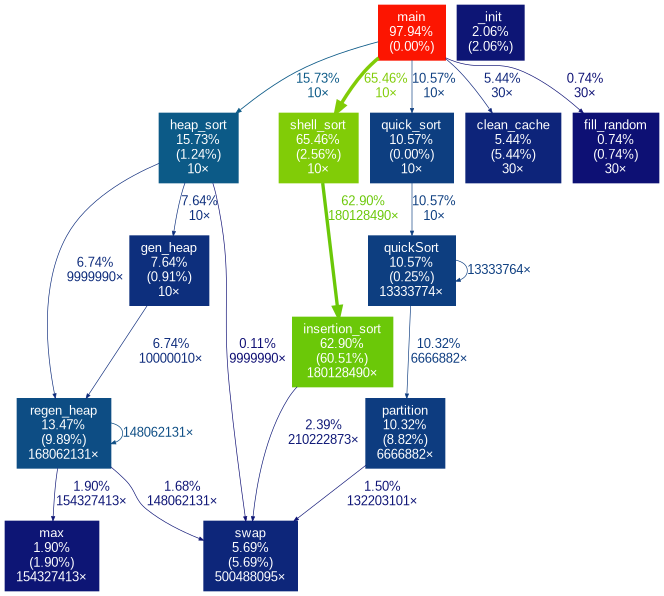
\includegraphics[width=1.4\textwidth]{data/graph.png}}

\newpage
\section{Análise}
A maior parte do tempo de execução foi para os algoritmos de ordenação, correspondente à \(91.76\%\) do tempo total. 

Dentre os algoritmos de ordenação usados, temos 3 algoritmos com complexidade média esperada de \(O(n\cdot log(n))\).
Como vemos, o shell sort consumiu o maior tempo de execução, dentro da sub-rotina de insertion sort, isso ocorreu pois é difícil estabelecer a complexidade média real do shell sort, sendo necessária uma análise cuidadosa do gap utilizado \footnote{\url{https://en.wikipedia.org/wiki/Shellsort}}, por este motivo não é fácil criar técnicas que garantam a complexidade com grande probabilidade, como no caso do uso da mediana de três para a escolha do pivô do quicksort, \citep{leiserson1994introduction}, que garante uma complexidade média de \(O(n\cdot log(n))\). 

O quicksort obteve um resultado melhor que o heap sort, de forma não surpeendente, pois no quicksort são utilizados ponteiros que se cruzam; Os dados acessados estão sempre sequenciais na memória, contribuindo para a localidade da cache, enquanto no heap sort pode haver, em uma determinada iteração, em um mesmo sub-vetor, dois dados que estão muito distantes na memória, além disso os loops internos do quicksort são menores, o que reflete um tempo menor de execução das sub-rotinas, como fica explicíto na comparação com as sub-rotinas do heap sort. Vale dizer também que o quicksort utiliza um espaço de memória com tamamho da ordem de \(O(log(n))\) de forma implícita na pilha, no momento da recursão e é instável.

\section{Conclusão}

Podemos concluir que o algoritmo quicksort apresentou melhor tempo de execução, devido à suas características de um melhor uso de localidade de cache, um espaço adicional de memória e ser um algoritmo instável, o heap sort fica em segundo lugar, sendo ele, verdadeiramente um sort in-place (sem uso de espaço auxiliar), e o shell sort fica em terceiro lugar, por usar uma sub-rotina com complexidade da ordem de \(O(n^2)\), mesmo que com uma execução que tenda para o melhor caso \(O(n)\) pelo uso de gaps iniciais grandes (que, mesmo com complexidade mais alta, terão um n pequeno).

\bibliographystyle{apalike}
\bibliography{bib.bib}

\end{document}
